\subsection{Introduction}
\begin{frame}{Cross-Validation}{Introduction}

\begin{itemize}
    \item Recall the \textit{test error rate} and the \textit{training error rate}: \pause
    \begin{enumerate}
        \item Test error rate: Average error that results from using a model to predict the response on a \textbf{new observation}. \pause
        \item Training error rate: calculated by applying the model to the observations used in its training. \pause 
    \end{enumerate}

    $\rightarrow$ \textcolor{blue}{We are interested in the model which results in a lowest test error}. \pause \\
    $\rightarrow$ But a test dataset is not always available. \pause

    \item To deal with this, we instead consider \textbf{holding out} a subset of the training observations from the fitting process. \pause \\ 
    
    \item Then we apply the model to those held-out observations to obtain the test error rate. 
    
\end{itemize}
    
\end{frame}

\subsection{The validation set approach}
\begin{frame}{Cross-validation}{The validation set approach}
    
\begin{enumerate}
    \item Randomly divide the available set of observations into two parts: a training set and a validation set. \pause
    \item Fit the model on the training set. \pause
    \item Predict the responses for the observations in the validation set. \pause
    \item The resulting validation set error rate provides an estimate of the test error rate. \pause
\end{enumerate}

\begin{block}{\textbf{Drawbacks:}}
\begin{itemize}
    \item The validation estimate of the test error rate can be highly variable:  \pause
    \\ $\rightarrow$ Random splitting.  \pause

    \item Statistical methods tend to perform worse when trained on fewer observations: \pause \\  The validation set error rate may tend to overestimate the test error rate for the entire data set. \pause 
\end{itemize}

    
\end{block}

We will present cross-validation, a method that addresses these two issues. 
\end{frame}

\subsection{Leave-one-out cross-validation}
\begin{frame}{Cross-Validation}{Leave-one-out cross-validation}

\begin{itemize}
    \item Split the set of observations into two parts: \pause 
    \begin{enumerate}
        \item A single observation $(x_1 , y_1 )$, used as the validation set. \pause
        \item The remaining observations $\{(x_2 , y_2 ), \cdots , (x_n, y_n )\}$, used as the training set. \pause
    \end{enumerate}
    
    \item Fit the model on the $n - 1$ training observations. \pause 
    
    \item Make a prediction $\hat{y}_1$ for the excluded observation, using its value $x_1$. \pause

    \item Since $(x_1 , y_1)$ was not used in the fitting process, $MSE_1 = (y_1 - \hat{y}_1 )^2$ provides an approximately \textbf{unbiased} estimate for the test error. \pause 
    
    \item However, it is a poor estimate because it is highly variable. \pause \\  
    $\rightarrow$ It is based upon a single observation $(x_1 , y_1)$. \pause

    \item Repeating this approach $n$ times produces $n$ squared errors. \pause \\
    $\rightarrow$  Select $(x_2 , y_2 )$ as the validation data, train the model on $\{(x_1 , y_1 ), (x_3 , y_3 ) \cdots , (x_n, y_n )\}$ and compute $MSE_2 = (y_2 - \hat{y}_2 )^2$. \pause
 
    \begin{equation}
        CV_{n} = \frac{1}{n} \sum_{i=1}^n MSE_i. 
    \end{equation}
    
\end{itemize}
    
\end{frame}


\begin{frame}{Cross-Validation}{Leave-one-out cross-validation}

\begin{figure}
    \centering
    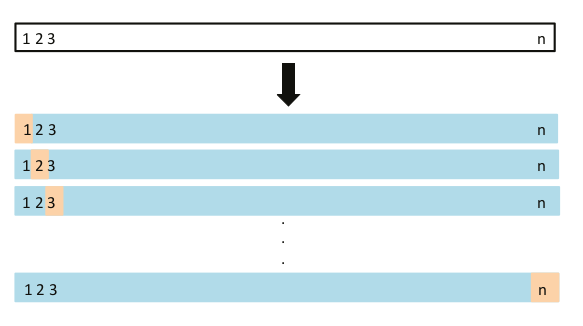
\includegraphics[height=4cm]{cross-val/l-o-o-cv.png}
\end{figure} \pause 

\begin{itemize}
    \item This approach has less bias than the validation set approach. \\ \pause  
    $\rightarrow$ Does not overestimate the test error rate as much as the validation set approach does. \pause 
    
    \item Performing LOOCV multiple times will always yield the same results. \\ \pause 
    $\rightarrow$ There is no randomness in the training/validation set splits.
\end{itemize}
    
\end{frame}


\begin{frame}{Cross-Validation}{Leave-one-out cross-validation}

\begin{block}{\textbf{Drawbacks:}}

    \begin{itemize}
        \item LOOCV has the potential to be expensive to implement, since the model has to be fit $n$ times. \pause 

        \item This can be very time consuming if $n$ is large, and if
each individual model is slow to fit.
    \end{itemize}

\end{block}

    
\end{frame}

\subsection{k-fold cross-validation}
\begin{frame}{Cross-Validation}{k-Fold cross-validation}

\begin{enumerate}
    \item Randomly divide the set of observations into $k$ groups, or folds, of approximately equal size.  \pause 
    
    \item The first fold is treated as a validation set, and the method is fit on the remaining $k - 1$ folds.  \pause 
    
    \item The mean squared error, $MSE_1$ , is then computed on the observations in the held-out fold.  \pause 
    
    \item Repeated this procedure $k$ times; each time. \\ \pause 
    $\rightarrow$ A different group of observations is treated as a validation set. \\ \pause
    $\rightarrow$ This process results in $k$ estimates of the test error, $MSE_1 , MSE_2 , \cdots , MSE_k$.  \pause 
    
    \item The k-fold CV estimate is computed by averaging these values.

    \begin{equation}
        CV_{(k)} = \frac{1}{k} \sum_{i=1}^k MSE_i. 
    \end{equation}
\end{enumerate}
    
\end{frame}

\begin{frame}{Cross-Validation}{k-Fold Cross-Validation}

\begin{figure}
    \centering
    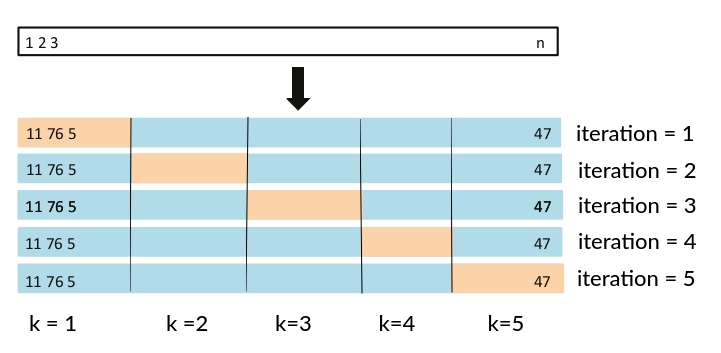
\includegraphics[height=4cm]{cross-val/kfold.png}
\end{figure} \pause 


\begin{itemize}
    \item LOOCV is a special case of k-fold CV in which $k$
is set to equal $n$. \pause 
    \item In practice, one typically performs k-fold CV using $k = 5$ or $k = 10$. \pause 
    \item What is the advantage of using $k = 5$ or $k = 10$ rather than $k = n$? \pause \\
    $\rightarrow$ The most obvious advantage is computational. 
    
\end{itemize}
    
\end{frame}


\subsection{Bias-variance trade-off for k-fold cross-validation}
\begin{frame}{Cross-Validation}{Bias-variance trade-off for k-fold cross-validation}

Summarizing, 

\begin{itemize}
    \item Validation set approach can lead to overestimates of the test error rate. \pause \\
    $\rightarrow$ The training set used to fit the model contains only half the observations of the entire data set. \pause 

    \item LOOCV will give approximately unbiased estimates of the test error. \pause \\
    $\rightarrow$ Each training set contains $n - 1$ observations, almost as many as the full number of observations. \pause

    \item k-fold CV for $k = 5$ or $k = 10$ will lead to an intermediate level of bias. \pause \\ 
    $\rightarrow$ Each training set contains approximately $(k - 1)n/k$ observations. \pause 

\end{itemize}


\textcolor{blue}{For bias reduction, LOOCV is to be preferred to k-fold CV.} 

\end{frame}

\begin{frame}{Cross-Validation}{Bias-variance trade-off for k-fold cross-validation}
    
However, there is some problems with LOOCV: 

\begin{itemize}
    \item Has higher variance than does k-fold CV with $k < n$. \pause 
    \item We are using almost identical training observations to then average the outputs. \pause \\ 
    \item These outputs are highly correlated with each other! \pause 

\end{itemize}

In contrast, when using k-fold CV with $k < n$, \pause 

\begin{itemize}
    \item We split the data into folds and then average the outputs. \pause 
    \item The outputs are somewhat less correlated with each other. \pause 
\end{itemize}

The mean of \textcolor{blue}{many highly correlated} quantities has higher variance than does the mean of many quantities that are not
as highly correlated. \pause 

\begin{block}{Bias-variance trade-off}
    \begin{itemize}
        \item Given these considerations, one performs k-fold cross-validation using $k = 5$ or $k = 10$. \pause 
        \item These values have been shown to yield test error rate that suffer neither from excessively high bias nor from very high variance.
    \end{itemize}
\end{block}


    
\end{frame}

\subsection{Cross-validation on classification problems}
\begin{frame}{Cross-validation on classification problems}

\begin{itemize}
    \item Cross-validation can also be a very useful
approach in the classification setting when $Y$ is qualitative. \pause

    \item In this setting, cross-validation works just as described earlier in this chapter. \pause 
    
    \item The only difference is that rather than using MSE to quantify test error, we instead use the number of misclassified observations. \pause 

    \item \textbf{For LOOCV}:

    \begin{equation*}
        CV_{(n)} = \frac{1}{n} \sum_{i=1}^n \text{Err}_i 
    \end{equation*} \pause
    
    \item \textbf{For k-fold CV}:

    \begin{equation*}
        CV_{(k)} = \frac{1}{k} \sum_{i=1}^n \text{Err}_i 
    \end{equation*}

    where $\text{Err}_i = I(y_i \not = \hat{y}_i)$ \pause
        
    \end{itemize} 
    
    
\end{frame}